\chapter{Theoretical background }\label{sec:theory}

\section{The learning framework}

Statistical learning theory encompasses the mathematical framework used to
study generalization in machine learning
\cite{n.vapnikNatureStatisticalLearning2000}.
In this formalism, the goal
is to learn a target function $f^*: \mathcal{X} \longmapsto \mathcal{Y}$ 
by means of an approximated function $f \in \mathcal{F}$ using a 
finite set of observations. 

\begin{definition}[Supervised dataset]\label{def:dataset}
    Let $\mathcal{X}$ and $\mathcal{Y}$ be
    the input and output spaces of the target function $f^*$, respectively. Let $X$ 
    be a random variable associated with a measure of probability in $\mathcal{X}$, 
    and let $\underbar{X} = (X_1, ..., X_N) \overset{\text{iid}}{\sim} X$ be a $N$-sized (simple)
    random sample of $X$ 
    \cite{casellaStatisticalInference2002}.
    A supervised dataset $D$ is a realization
     $\bm{x} \sim \underbar{X}$ paired with its output values under the 
     target function mapping.

    $$
    D = (\bm{x}, f^*(\bm{x})) = \{(x_n, f^*(x_n))\}_{n \in [N]}
    $$

    $\mathcal{D}$ will represent the class of supervised datasets generated from $\underbar{X}$.
\end{definition}

The quality of the approximation can be measured with the expected risk $\mathcal{R}(f)$:

$$
\mathcal{R}(f)=\mathbb{E}_{X} [\mathcal{L}(f(x),f^\star(x))]
$$

where $\mathcal{L}: \mathcal{Y} \times \mathcal{Y} \to \mathbb{R}$ denotes a loss function. 
The Glivenko-Cantelli theorem allows us to estimate the expected risk 
with its empirical (plug-in) analogous when $N$ is large 
enough \cite{gutIntermediateCourseProbability2009}.

\begin{definition}[Empirical risk]\label{def:erm}
    Let $D$ and $\mathcal{L}$ be the dataset and loss function of our problem, respectively. 
    The empirical risk of $f \in \mathcal{F}$ computed on $D$ is defined as

    $$
    \hat{\mathcal{R}}_D(f)=\frac{1}{N}\sum_{n=1}^{N}\mathcal{L}(f(x_{n}),f^{\star}(x_{n})).
    $$
\end{definition}

Training, therefore, amounts to minimizing the empirical risk over the function class $\mathcal{F}$:

$$
\text{ERM}_D = \hat{f}_D = \min_{f \in \mathcal{F}} \hat{\mathcal{R}}_D(f).
$$

The best learning algorithm will be that achieving the lowest generalization error
under sampling randomness, which is estimated as the empirical risk 
on a different dataset $D' \in \mathcal{D}$. \\

It can be shown that generalization 
error is ultimately linked to the complexity of the function class. 
The definition of complexity depends 
on the nature of the problem, but intuitively measures the cardinality of the
subset of $\mathcal{F}$ that the algorithm is able to represent. A complex or 
high-capacity algorithm will be able to represent a larger subset 
of $\mathcal{F}$ and achieve a low empirical error, but will be also
prone to overfitting to the specific learning realization thus yielding 
a higher generalization error \cite{n.vapnikNatureStatisticalLearning2000}. \\

As a general principle, the inductive bias of the algorithm (i.e. the set of constraints imposed on $\mathcal{F}$ during learning) should be aligned with
that of our target function
\cite{jimenezInductiveBiasDeep}. 
Given that more expressive classes are always preferred by optimization algorithms, the ERM
objective function is tweaqued to include a regularization term penalizing complexity.

\begin{definition}[Regularized empirical risk]\label{def:rrm}
    Let $\Omega: \mathcal{F} \to \mathbb{R}$ be a functional quantifying the complexity
    of the elements of the function class. The regularized empirical risk of $f \in \mathcal{F}$
    computed on dataset $D$ is defined as

    $$
    \hat{\mathcal{R}}_{\Omega}(f)=\hat{\mathcal{R}}(f) + \lambda \Omega(f),
    $$

    where $\lambda \in \mathbb{R}$ controls the trade-off between empirical risk and generalization error.

\end{definition}



\section{Learning with neural networks}

Neural networks are biologically-inspired machine learning models that consist of a set of 
nodes (neurons) organized in layers and connected by weighted edges
(synapses). Figure \ref{fig:nn_node} illustrates the transformation
performed within a single node
\cite{simonyanVeryDeepConvolutional2015,n.vapnikNatureStatisticalLearning2000,voulodimosDeepLearningComputer2018}. 

\begin{figure}[H]
    \centering
    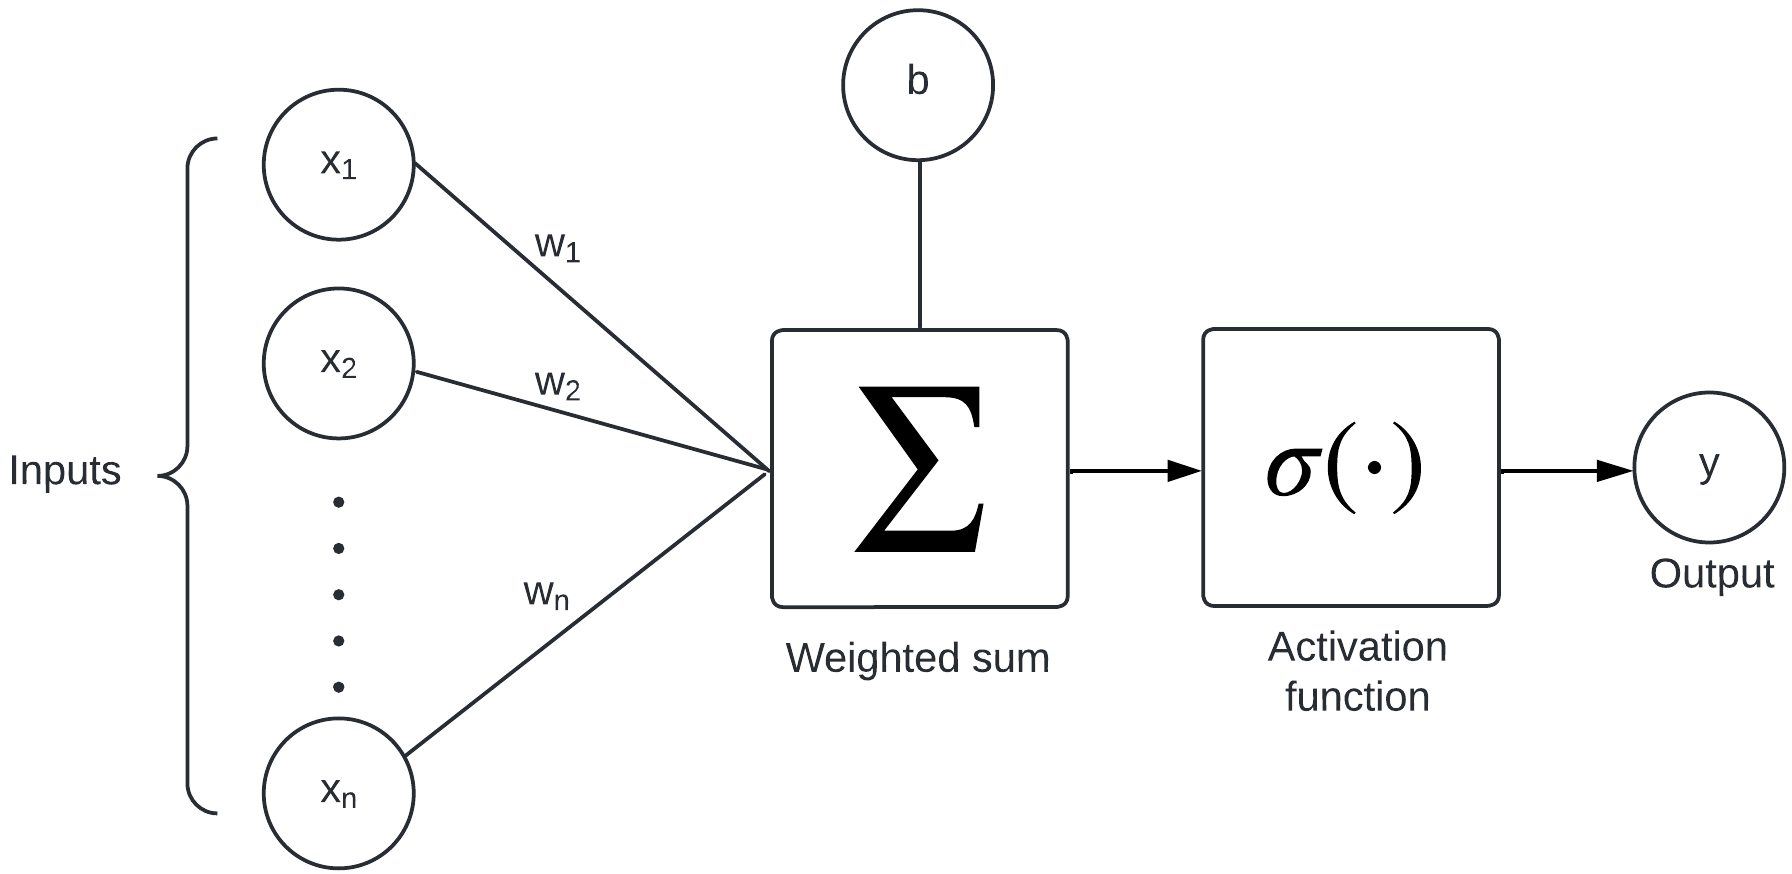
\includegraphics[width=0.6\textwidth]{img/theoretical_background/nn_unit.png}
    \caption{The output of a node is computed by applying a non-linear
    activation function $\sigma$ to the weighted sum of its inputs $\bm{x}$ plus
    a bias term $b$.}
    \label{fig:nn_node}
\end{figure}

Let $\bm{x}_k \in \mathbb{R}^{d_k}$ be the input to the layer $k \leq L$, and 
let $\bm{W} \in \mathbb{R}^{d_k \times d_{k+1}}$ be the $k$-th weight matrix. 
The output of the layer can be expressed as

$$
\bm{x}_{k+1} = \sigma_k(\bm{z}_{k+1}) = \sigma_k(\bm{W}_k^T \bm{x}_k + \bm{b}_k),
$$

where $\sigma_k$ is the non-linear activation function at layer $k$. We 
can therefore express the overall transformation of a neural network
as the composition of its layers:

$$
f_{\text{NN}}(\bm{x}) = \bigcirc_{k=0}^{L-1} \sigma_k(\bm{W}_k^T \bm{x} + \bm{b}_k) = f(\bm{x}; \gamma),
$$

where $\gamma \in \Gamma \subset \mathbb{R}^S$ represents the set of parameters of the network. In order to solve the learning problem, the optimization algorithm must navigate the non-convex loss
landscape towards the minimum of the empirical risk. This is computationally achieved 
by means of gradient-descent-based optimizers, which efficiently compute the
gradient over the parameters via the backpropagation algorithm 
\cite{rumelhartLearningRepresentationsBackpropagating1986}. In practice, more efficient
variations of gradient descent are used, such as stochastic gradient descent 
\cite{ruderOverviewGradientDescent2017} 
or the Adam optimizer 
\cite{kingmaAdamMethodStochastic2017}. \\


% \subsection{Backpropagation and gradient descent}

% Let $w_{ji}^{(k)}$ be the weight from node $j$ on layer $k-1$ to node $i$ on layer $k$. Let $a_i^{(k-1)}$ be the output of node $i$ on layer $k-1$ and let $z_j^{(k)} = \sum_{i=0}^{n_k - 1} w_{ji}^{(k)} a_i^{(k-1)} + b_k^{(k)}$ be 
% the linear input of node $j$ on layer $k$, so that $a_j^{(k)} = \sigma_j(z_j^{(k)})$ is the ouput from node $j$. We can compute the gradient of the loss $\mathcal{L}$ with respect to the weights by means of the chain rule as follows: 

% $$  
% \frac{\partial \mathcal{L}}{\partial w_{ji}^{(k)}} = \frac{\partial \mathcal{L}}{\partial a_{j}^{(k)}} \frac{\partial a_{j}^{(k)}}{\partial z_{j}^{(k)}} \frac {\partial z_{j}^{(k)}} {\partial w_{ji}^{(k)}} =
% \frac{\partial \mathcal{L}}{\partial a_{j}^{(k)}} \frac{\partial \sigma_j^{(k)}}{\partial z_{j}^{(k)}} a_i^{(k-1)}
% $$

% Given that the loss is computed as a function of the output of the network, all the edges from node $i$ of layer $k-1$ influence the loss value at that node:

% $$
% \frac{\partial \mathcal{L}}{\partial a_{i}^{(k-1)}} = \sum_{j=0}^{n_{k} - 1} \frac{\partial \mathcal{L}}{\partial a_{j}^{(k)}}  \frac{\partial a_{j}^{(k)}}{\partial z_{j}^{(k)}} \frac{\partial z_{j}^{(k)}}{\partial a_{i}^{(k-1)}} =
% \sum_{j=0}^{n_{k} - 1} \frac{\partial \mathcal{L}}{\partial a_{j}^{(k)}} \frac{\partial \sigma_j^{(k)}}{\partial z_{j}^{(k)}} w_{ji}^{(k)}
% $$

% All in all, we see that the same terms are required in different nodes to compute the gradient, making backpropagation algorithm very efficient. Equivalently, for the bias term:

% $$
% \frac{\partial \mathcal{L}}{\partial b_{j}^{(k)}} = \frac{\partial \mathcal{L}}{\partial a_{j}^{(k)}} \frac{\partial a_{j}^{(k)}}{\partial z_{j}^{(k)}} \frac {\partial z_{j}^{(k)}} {\partial b_{j}^{(k)}} = \frac{\partial \mathcal{L}}{\partial a_{j}^{(k)}} \frac{\partial \sigma_j^{(k)}}{\partial z_{j}^{(k)}}
% $$

% These derivatives are the components of the gradient vector that will be used to update the weights and biases of the network.

% $$
% w_{ji}^{(k)} = w_{ji}^{(k)} -\eta \frac{\partial \mathcal{L}}{\partial w_{ji}^{(k)}}
% $$

% $$
% b_{j}^{(k)} = b_{j}^{(k)} -\eta \frac{\partial \mathcal{L}}{\partial b_{j}^{(k)}}
% $$

% where $\eta$ is the learning rate. More efficient variations of gradient descent such as stochastic gradient descent or Adam are used in practice.


% \subsection{Loss landscape and parameter space}


A neural network architecture $\text{NN}$ can be expressed as a parametrization of the function space $\mathcal{F}$:

$$
    \begin{aligned}
        \text{NN}: \Gamma & \subseteq \mathbb{R}^{S} \longmapsto \mathcal{F}_{\Gamma} \\
        \gamma & \longmapsto f(\bm{x}; \gamma) = f_{\text{NN}}(\bm{x}),
    \end{aligned}
$$

where $\Gamma$ is the parameter space associated with this particular architecture. The functional
landscape $\mathcal{F}_{\Gamma}$ consists of all mappings $f(\gamma): \mathcal{X} \longmapsto \mathcal{Y}$ that 
that can be realized by some parameter configuration $\gamma \in \Gamma$. \\

The universal approximation theorem states that an arbitrarily wide architecture
is able to represent virtually any function, but it is an open challenge to theoretically describe which
complexity measure regulates generalization. A possible approach to this problem is to
study the geometry of the loss landscape, especially in the vicinity of local minima. For instance, 
connected flat minima are often linked to better generalization capabilities, as they
intuitively represent a robust region in the parametrization space and should be 
preferred over sharp minima
\cite{jimenezInductiveBiasDeep}. \\

In this work we will explore a different approach to the generalization problem, rooted on
a measure of generalization error that accounts for the implicit randomness of the data
generation process.

\section{Posterior agreement}

As mentioned at the start of the chapter, the input of learning algorithms are
datasets containing samples of a random variable $X$ with support $\mathcal{X}$. The implicit randomness embedded 
in the sampling process extends to the learning outcome of algorithms,
even when performing a deterministic set of operations
\cite{buhmannDataScienceAlgorithms2022}. 
An alternative intuition of 
generalization arises from this perspective, in the sense that a good algorithm should be
expected to learn the same function when trained on different realizations 
of the same experiment; that is, when datasets are drawn from the same random vector 
but entail different instantiations of the noise associated with the sampling process. \\

A regularization principle is derived from this intuition and can be formalized as a
generalization-complexity trade-off by defining generalization as the robustness or stability
of the learned function to sampling noise. A suitable measure of complexity in this framework
is the informativeness of the function, which represents its ability to learn the patterns in the
data while filtering out the noise. The more expressive (i.e. complex) a function class is,
the higher will be the estimated information content of the data. If the information content is
underestimated, the approximated function will lack the capacity to learn some patterns in
the data, whereas if informativeness is overestimated, it will overfit to the noise and 
thus not generalize to different realizations of the experiment
\cite{chehreghaniInformationTheoreticModel,buhmannInformationTheoreticModel,buhmannInformationTheoreticModel2010}. \\

The robustness-informativeness regularization principle can be enforced from the set 
of outputs of the learned model, when both the distribution of the data over the support 
and the sampling randomness associated to its measurement are accounted for. This section 
will formalize this principle and derive an expression for the minimization of
the generalization error under this framework.

\begin{definition}[Data distribution]
    The (simple) random sample $\underbar{X} \overset{\text{iid}}{\sim} X$ has a probability distribution
    described by the density function $f_{\underbar{X}}$:

    $$
     f_{\underbar{X}} = \prod_{n=1}^{N} f_{X}(x).
    $$

    We will use $\mathbf{P}_{X}$ to refer to the empirical approximation of this distribution; 
    that is, to the distribution of samples in a dataset $D$ drawn from $\underbar{X}$:

    $$
    \mathbf{P}_{X} = \frac{1}{N} \sum_{n=1}^{N} \delta(x - x_n).
    $$

\end{definition}

\begin{definition}[Sample]
    Let $X$ be a random variable associated with a measure of probability
    in $\mathcal{X}$. 
    Let $\tau \in \mathbb{T}$ be a source of randomness allowed
    by such measurement.
    The set of transformations $\mathbb{T}$ is composed
    of the possible experimental conditions for the data sampling 
    process from $X$. The dependency of measurement 
    realizations $\bm{x} \sim \underbar{X}$ on experimental conditions 
    will be captured by index $\tau$, and we will implicitly consider sample
    
    $$
        \bm{x} := \tau \circ \bm{x}
    $$

    to be a realization of experiment $\underbar{X} \overset{\text{iid}}{\sim} X$ under conditions $\tau$. Given the stochastic
    nature of $\tau$, we will also refer to it as noise instantiation.
\end{definition}

These concepts will allow us to quantify the nature of the randomness that we are enforcing
models to be invariant to. A dataset drawn from $\underbar{X}$ entails a 
noise instantiation $\tau$ that is not observed, which implies that we don't have access to the 
true information content of the data that derives from its true distribution $f_{\underbar{X}}$.

\subsection{Posterior distribution}

%The approximating function $f \in \mathcal{F}$ has been defined as a mapping 
%$\mathcal{X} \longmapsto \mathcal{Y}$, in the sense that an observation $x \in \mathcal{X}$ is mapped to
%a prediction $f(x) \in \mathcal{Y}$. A subtle abuse of notation will be made when considering
%5$f$ to be a 

% THIS IS NOT TRUE
% The data informativeness approximation entailed by the model depends fundamentally
% on the nature of the learning problem, since different tasks will demand different levels of
% informativeness. In the supervised learning framework, we can analogously consider a target 
% information content, which refers to the informativeness of the true mapping of the dataset 
% class. The quality of the approximation will be thus given by the alignment of the informativeness
% attributed to the data with the target information content, which .


% Following this intuition, the robustness of a model will be given by 
% its stability under different noise instantiations,  which is maximum when samples containing the same information are mapped to the same 
% output.

\begin{definition}[Hypothesis class]
    Let $\mathcal{D}$ be the class of datasets generated from $N$-sized realizations of $\underbar{X}$. 
    A data science algorithm learns a function $f$ implementing the following mapping:

    $$
    \begin{aligned}
        f: \mathcal{D} & \longmapsto \Theta \\
        \bm{x}  & \longmapsto (f(x_1), \dots, f(x_N)) = \theta.
    \end{aligned}
    $$

    The hypothesis class $\Theta$ is the output space of hypothesis representing all 
    possible outcomes of a function $f$ learned on a dataset sampled from $\underbar{X}$
    \cite{buhmannDataScienceAlgorithms2022}.

\end{definition}

Intuitively, this framework interprets complexity from the perspective of the possible
set of outcomes of the function, rather than the function class itself. It can be argued
that both perspectives are equivalent, in the sense that any function class can be 
ultimately mapped to a specific hypothesis space $\Theta$. Nevertheless, the underlying transformation is not
homeomorphic in general, and more suitable generalization regularization
constraints can be defined in $\Theta$, especially when dealing with intractable
function classes $\mathcal{F}_{\Gamma}$ represented by deep neural networks. \\

For instance, complexity in the hypothesis class can be associated to the nature of the
randomness displayed by $X$. Ideally, too restrictive hypothesis classes that lack desirable
hypothesis for some realization $\bm{x} \sim \underbar{X}$ should be avoided, and also those hypothesis
classes containing unrealizable elements (i.e. hypothesis that are not outcome of
any possible realization of the experiment). A richness condition for the construction of $\Theta$ 
can thus be postulated following this intuition. \\

\begin{definition}[Richness condition]
    $\Theta$ should stem from a
    sufficiently rich set of experimental conditions $\mathbb{T}$ such that every hypothesis $\theta \in \Theta$
    is the outcome of some realization $\bm{x} \sim \underbar{X}$.

    $$
    \forall \theta, \exists \tau \in \mathbb{T} \text{ such that } f(\bm{x}) = \theta
    $$
\end{definition}


Since we assume a mapping $f$ and a data distribution $\mathbf{P}_{X}$, we can describe
the randomness of the hypothesis outcome conditioned on the distribution of the data.

\begin{definition}[Posterior]\label{def:posterior}
    Let $\mathfrak{P}^f$ be a probability distribution family under consideration.
    A probability distribution over the hypothesis class can be defined as a 
    conditional distribution given an realization $\bm{x} \sim \underbar{X}$. 
    We will refer to this distribution as the posterior over $\Theta$ under $f$:

    $$
        \begin{aligned}
            \mathbf{P}^f: \mathcal{D} \times \Theta & \longmapsto \mathbb{R} \\
            (\bm{x}, \theta) & \longmapsto \mathbf{P}^f (\theta \mid \bm{x}).
        \end{aligned}
    $$

    The posterior $\mathbf{P}^f \in \mathfrak{P}^f$ establishes the stochastic relation between data realizations and hypotheses.
    
\end{definition}

Using these definitions we can operate over $\Theta$ within the framework of probability 
theory. For instance, we can obtain the (prior) probability of a hypothesis to be
selected by $f$ as

$$
 \Pi^f (\theta) = \mathbb{E}_{\mathbb{T}} \; \mathbf{P}^f (\theta \mid \tau) = \mathbb{E}_{\underline{X}} \; \mathbf{P}^f (\theta \mid \bm{x}),
$$

from which we can derive a probabilistic version of the richness condition, where a limit
case can be imposed with exactly one experiment per hypothesis, leading to a uniform prior

$$
\Pi^f (\theta) = |\Theta|^{-1}
$$

when the hypothesis class is finite. Within this framework, selecting suitable hypothesis classes amounts to selecting
posterior distributions that yield a higher probability to the desired subset of hypothesis. This
is the leading principle that will guide the derivations that follow.

\subsection{Generalization error}

In order to define a robustness-based generalization error, we will proceed in an
analogous way as we did in the previuous section. We will consider datasets $D', D'' \in \mathcal{D}$
each arising from a different sampling realization $\bm{x}', \bm{x}'' \sim \underbar{X}$, respectively. 
Both realizations are independent and they differ in the implicit noise entailed by
their measurement:

$$
    \mathbf{P}_{\bm{x}', \bm{x}''} = \mathbf{P}_{\bm{x}'} \mathbf{P}_{\bm{x}''}.
$$

Two posterior selection principles are derived from the robustness-informativeness trade-off:
\vspace{-2mm}
\begin{description}
    \item[P1] Posteriors should be expressive enough to cover the realizable subset of the hypothesis space.
    \vspace{-3mm}
    \item[P2] Equally likely inputs drawn from the same experiment should yield similar sets of hypothesis.
\end{description}

\begin{definition}[Description length]
    Let $\mathcal{F}_{\Gamma}(\cdot)$ be the function class containing all functions 
    represented by a parametrization $\Gamma$. Let $\mathbf{P}_{\Gamma}$ be the
    universal distribution relative to $\mathcal{F}_{\Gamma}$ fulfilling the minimum
    description length principle. The description length of a function $f_\gamma \in \mathcal{F}_{\Gamma}$ 
    is defined as the number of bits required to encode its parameters
    \cite{grunwaldMinimumDescriptionLength2019}.
    The code length of the argument of such distribution is

    $$
    \text{DL}_{f_{\gamma}}(\cdot) = -\log f_{\gamma}(\cdot).
    $$
\end{definition}

The quality of the represented function $f$ will be measured by the description
length of its posterior \cite{buhmannDataScienceAlgorithms2022}, and 
thus a loss function can be defined as follows:

$$
    \ell (\theta, \bm{x}) = - \log \mathbf{P}^f (\theta \mid \bm {x}).
$$

Given that description length also accounts for the complexity of the hypothesis
class and not only its generalization capabilities, we will normalize loss values by
dividing by the description length of the prior:

$$
    - \log \Pi^f (\theta) = - \log \mathbb{E}_{\underline{X}} \mathbf{P}^f (\theta \mid \bm{x}).
$$

\begin{definition}[Generalization error]
    Let $\bm{x'}$ and $\bm{x''}$ be realizations of $\underbar{X}$.
    Let $\Theta$ be the hypothesis class represented by $f$ given $\underbar{X}$. 
    The generalization error is defined as the out-of-sample description length:

    $$
        \mathcal{G}_{\mathcal{X}} = \mathbb{E}_{\mathbf{P}^f(\bm{x}', \bm{x}'')} \mathbb{E}_{\mathbf{P}^f( \theta \mid \bm{x}')} \left[ - \log \frac{\mathbf{P}^f(\theta | \bm{x}'')}{\Pi^f (\theta)} \right].
    $$
    
\end{definition}

It amounts to the expected loss over the normalized posteriors on the validation data
$\bm{x}''$ weighted over the posterior distribution on the training data $\bm{x}'$.
Intuitively, a lower generalization error is achieved when good quality hypothesis
on $\bm{x}''$ are likely to be drawn from $\bm{x}'$. 


\begin{lemma}[Posterior agreement]\label{lemma:pa}
    The generalization error $\mathcal{G}_{\mathcal{X}}$ is non-negative and has a lower bound $-\mathcal{J}$. 
    \textcolor{blue}{We define $\mathcal{J}$ as the posterior agreement.}
\end{lemma}
\begin{proof}
    $$
    \begin{aligned}
        \mathcal{G}_{\mathcal{X}} & \geq \mathbb{E}_{\mathbf{P}^f(\bm{x}', \bm{x}'')}\left[-\log \left(\mathbb{E}_{\mathbf{P}^f( \theta \mid \bm{x}')} \frac{\mathbf{P}^{f}\left(\theta \mid \bm{x}''\right)}{\Pi^{f}(\theta)}\right)\right] \\
        & = \textcolor{blue}{\boxed{\mathbb{E}_{\mathbf{P}^f(\bm{x}', \bm{x}'')} \left[-\log \left(\sum_{\theta \in \Theta} \frac{\mathbf{P}^{f}\left(\theta \mid \bm{x}'\right) \mathbf{P}^{f}\left(\theta \mid \bm{x}'' \right)}{\Pi^{f}(\theta)}\right)\right] = -\mathcal{J}}} \\
        & \geq-\log \left(\mathbb{E}_{\mathbf{P}^f(\bm{x}', \bm{x}'')} \mathbb{E}_{\mathbf{P}^f( \theta \mid \bm{x}')} \mathbb{E}_{\mathbf{P}^f(\theta \mid \bm{x}'')} \frac{\mathbf{P}^{f}\left(\theta \mid \bm{x}''\right)}{\Pi^{f}(\theta)}\right)=0,
    \end{aligned}
    $$

where Jensen's inequality has been applied twice to the convex function $-\log(\cdot)$. \\

\end{proof}

\subsection{Maximum posterior agreement}

The maximum posterior agreement criterion, which follows 
from Lemma \ref{lemma:pa}, can be formalized as an optimization problem over the 
function class.

\begin{definition}[Kullback-Leibler divergence]
    Let $\mathbf{P}$ and $\mathbf{Q}$ be two probability distributions over the same support $\Theta$. 
    The Kullback-Leibler divergence of $Q(\theta)$ relative to $P(\theta)$ is defined as

    $$
    \text{KL}(\mathbf{P}(\theta) \parallel \mathbf{Q}(\theta)) = \mathbb{E}_{\mathbf{P}(\theta)} \left[ \log \frac{\mathbf{P}(\theta)}{\mathbf{Q}(\theta)} \right].
    $$

\end{definition} 

\begin{definition}[Cross-entropy]
    Let $\mathbf{P}$ and $\mathbf{Q}$ be two probability distributions over the same support $\Theta$. 
    The cross-entropy of $Q(\theta)$ relative to $P(\theta)$ is defined as

    $$
    \mathcal{H}_{\mathbf{P}, \mathbf{Q}} = - \mathbb{E}_{\mathbf{P}(\theta)} \log \mathbf{Q}(\theta)
    $$

\end{definition}

\begin{definition}[Posterior agreement criterion]\label{def:pa}
    The posterior agreement model-selection criterion is defined as follows.

    $$
    \begin{aligned}
        \sup_{\mathcal{F}} & \; \mathcal{J} \\
        \text{s.t.} & \; \text{KL}(\mathbf{\Pi}^f(\theta) \parallel |\Theta|^{-1}) \leq \xi,
    \end{aligned}
    $$
    
    where $\xi \in \mathbb{R}$ represents a small allowed deviation from uniformity in the prior.
\end{definition}

\begin{theorem}
The optimal $\mathbf{P}_{*}^f$ maximizing the posterior agreement criterion defines a lower bound
in the generalization error $\mathcal{G}_{\mathcal{X}}$ under the richness condition:

$$
    \inf_{\mathcal{F}} \mathcal{G}_{\mathcal{X}} \geq -\sup_{\mathcal{F}} \mathcal{J}.
$$
\end{theorem}

\begin{proof}
    We consider the lagrangian formulation of the generalization error minimization problem 
    and apply Lemma \ref{lemma:pa}.

    $$
    \begin{aligned}
        & \inf_{\mathcal{F}} \left \{ \mathcal{G}_{\mathcal{X}} + \alpha \text{KL} (\mathbf{\Pi}^f(\theta)) \parallel |\Theta|^{-1} \right \} \\
        = & \; \inf_{\mathcal{F}} \left \{ \mathcal{G}_{\mathcal{X}} + \alpha \mathbb{E}_{\mathbf{\Pi}^f(\theta)} \log \mathbf{\Pi}^f(\theta) + \alpha \mathbb{E}_{\mathbf{\Pi}^f(\theta)} \log |\Theta| \right \} \\
        \geq & \; \alpha \log |\Theta| + \inf_{\mathcal{F}} \left \{ \alpha \mathcal{H}_{\mathbf{\Pi}^f} \right \} - \sup_{\mathcal{F}} \left \{ \mathcal{J} \right \} \\
        \geq & \; - \sup_{\mathcal{F}} \mathcal{J}
    \end{aligned}
    $$

    The last inequality follows from the fact that the entropy does not exceed the log-cardinality
    of the hypothesis class:

    $$
    \mathcal{H}_{\mathbf{\Pi}^f}(\theta) \leq \log |\Theta|, \;\; \forall \mathbf{\Pi}^f.
    $$
\end{proof}




